%%%%%%%%%%%%%%%%%%%%%%%%%%%%%%%%%%%%%%%%%%%%%%%%%%%%%%%%%%%%%%%%%%%
%%%%%%%%%%%%%%%%%%%%%%%%%%%%%%%%%%%%%%%%%%%%%%%%%%%%%%%%%%%%%%%%%%%
\chapter{Fundamentação Teórica} \label{cap:fund}
%%%%%%%%%%%%%%%%%%%%%%%%%%%%%%%%%%%%%%%%%%%%%%%%%%%%%%%%%%%%%%%%%%%
%%%%%%%%%%%%%%%%%%%%%%%%%%%%%%%%%%%%%%%%%%%%%%%%%%%%%%%%%%%%%%%%%%%
    
    É uma análise comentada sobre o que já foi publicado sobre o assunto da pesquisa, buscando mostrar os pontos de vista convergentes e divergentes entre os autores. Traça-se um quadro teórico e elabora-se a estruturação conceitual que subsidiará o desenvolvimento  30 da pesquisa. A revisão de literatura permitirá um mapeamento de quem já escreveu e o que já foi escrito sobre o assunto ou o problema de pesquisa.

	Teste de Alguma abreviatura: \abreviatura*{CA}{corrente alternada}.
	
	\begin{figure}[H]
		\centering
		\caption{Um exemplo de figura}
		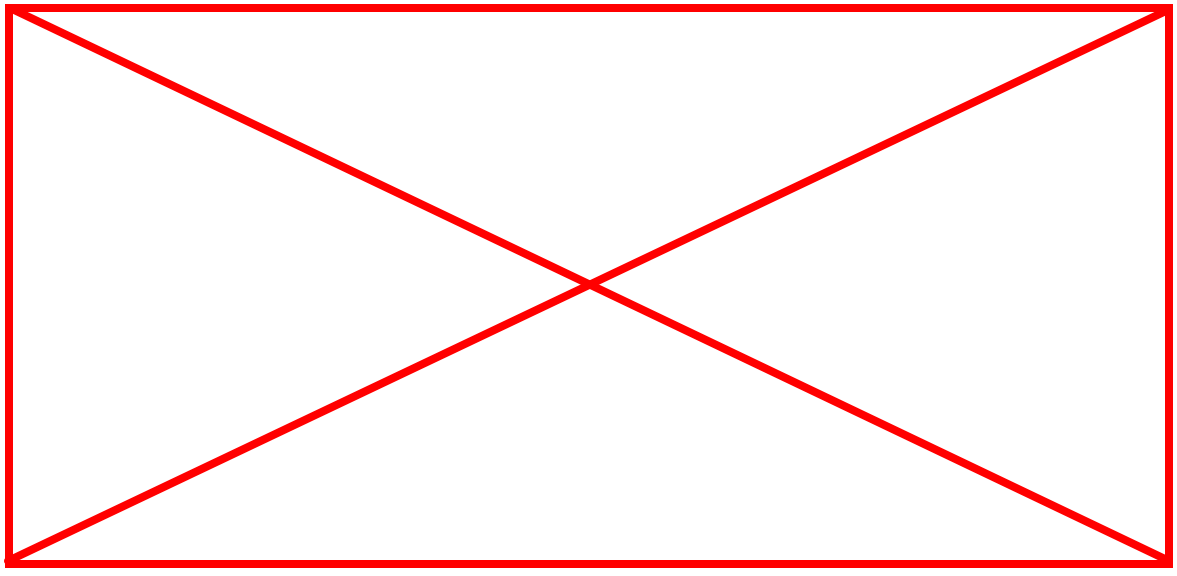
\includegraphics[width=\textwidth,height=240px,keepaspectratio]{pdf/noimage.png}
		\label{fig:esquematico_cbi}
		\indentedfont[15.2cm]{Elaboração própria (2021)}
	\end{figure}

	Alguns exemplos de equações:
	
	\[
		\binom{m+n}{m} = 
		\frac{(m+n)!}{m!n!} = 
		\frac{
			\overbrace{
				(m+n)(m+n-1)\cdots(n+1)
			}^{\clap{$m$ factors}}
		}{
			\underbrace{
				m(m-1)\cdots 1
			}_{\clap{$m$ factors}}}
	\]
	
	\begin{equation}
		\hat{x} = \hat{y} + a
	\end{equation}
	
	\begin{subequations}\label{eq-group1}
		\begin{align}
			\label{eq-lalala}
			\dot{x}
			&=	\begin{bmatrix}
				\dot{x_1} \\
				\dot{x_2} \\
				\dot{x_3} \\
			\end{bmatrix} 
			=	\begin{bmatrix}
				\dot{v_{C_1}} \\
				\dot{v_{C_2}} \\
				\dot{v_{C_3}} \\
			\end{bmatrix}
			=	\overbrace{
				\begin{bmatrix}
					0 & 559.44 & 0 \\
					-21.01 & -100.93 & 21.01 \\
					0 & 0 & -666.67
			\end{bmatrix}}^{A} x
			+	\overbrace{
				\begin{bmatrix}
					0 \\
					0 \\
					666.67
			\end{bmatrix}}^{B} u \\
			\label{eq-ssplanta_final}
			y
			&=	\overbrace{
				\begin{bmatrix}
					1 & 0 & 0 \\
			\end{bmatrix}}^{C} x
			+	\overbrace{
				\begin{bmatrix}
					0
			\end{bmatrix}}^{D} u
		\end{align}
	\end{subequations}